\chapter{Clock System}

\section*{Aufgabe 5}

\paragraph*{}
Für die Lösung dieser und der nachfolgenden Aufgabe, war es nicht nötig ein Programm zu schreiben, wir konnten die Werte der erfoderlichen Regsiter über den Flasher direkt modfizieren. Gleichzeit massen wir mit einem angschlossenen Ozziloskop die aktuelle Frequenz des MCLK-Taktes, die über P5.5 nach aussen geführt wird, wenn die P5SEL und P5DIR entsprechend gesetzt sind.

\paragraph*{}
Unsere Ergebnisse finden sich in nachfolgender Tabelle: \\

\begin{tabular}{ p{4cm} | c | p{4cm} }\hline \hline
Clocksrv & DIVM-Bits & Frequenz \\ \hline
DCOCLK & 00 & 776,5 Khz \\ \cline{2-3}
DCOCLK & 01 & 388 Khz \\ \cline{2-3}
DCOCLK & 10 & 194,1 Khz \\ \cline{2-3}
DCOCLK & 11 & 97 Khz \\ \hline
XT2CLK & 00 & 7,37 Mhz \\ \hline
LFXT1CLK & 00 & 32,77 Khz \\ \hline
\end{tabular}

\paragraph*{}
Mit durch setzen des DCOR-Bits auf 1 wird ein externer Widerstand angeschlossen. Dies führt nach unseren Beobachtungen zu einem stabilieren Takt. Mit dem DIVM-Bits wird der Devisor gesteuert. Er er möglicht es Bruchteile der eigenlichen Tackquelle zu erhalten. 

\section*{Aufgabe 6}

\paragraph*{}
Durch unsere Messung konnten wir einen linearen Zusammenhang zwischen Strom und der Frequenz des MCLK-Taktes feststellen. Dies erscheint logisch unter der Annahme das ein Schaltvorgang konstant viel Strom benötigt, unabhänig von seiner Geschwindigkeit.

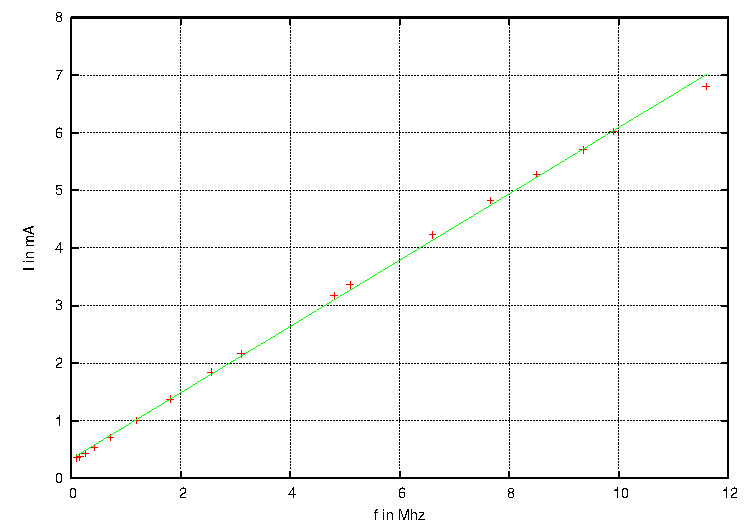
\includegraphics[width=\textwidth]{graphs/vfgraph.pdf}


\section*{Aufgabe 7}

\paragraph*{}
Um die gewünschten Einstellung zu treffen nutzen wir die Register {\em DCOCTL},{\em BCSCTL1} und {\em BCSCTL2}. Die genauen nötigen Einstellung ermittelten wir vorher nach dem try-and-error Prinzip.

\lstinputlisting[caption=aufgabe7.c]{src/aufgabe7.c}

\paragraph*{}
Anschließend konnten wir am angeschlossenen Ampermeter folgende Werte ermitteln: \\

\begin{tabular}{ c | c | c }\hline \hline
Frequenz & Stromverbrauch & Laufzeit mit 1100 mAh Batterie \\ \hline
4,096 kHz & 0,376 mA & 2926 h (ca. 122 Tage) \\ \hline
7,3728 MHz & 4,635 mA & 273 h (ca. 10 Tage) \\ \hline
\end{tabular}

\section*{Aufgabe 8}

\paragraph*{}
Da wir direkt auf den Prozessor zu greifen, und wir keine weiteren Programmflüsse auf dem Prozessor laufen haben, ist die Ausführungszeit eines Befehls gegeben als das Reziprok der Prozessorfrequent. Unter der Vorraussetzung das die Operation in einem Takt ab gearbeitet werden kann. 

\lstinputlisting[caption=aufgabe8.c]{src/aufgabe8.c}

\paragraph*{}
Für unsere spezille Aufgabe muss beachtet werden, das wir als Messergebnis eine Frequenz über zwei Zustandsänderungen erhalten.
Mittels des obigen Programms gelang es uns folgende Werte zu ermitteln: \\

\begin{tabular}{ c | c | c | c}\hline \hline
MCLK-Takt & berechnete Zeit & gemessene Frequenz & gemessene Zeit \\ \hline
4,096 kHz & $ 2,44 * 10^{-4} $ s &  & \\ \hline
7,3728 MHz & $ 1,37 * 10^{-7} $ s  & 262,9 hz & \\ \hline
\end{tabular}

\paragraph*{}
Die Abweichungen sind vermutlich darauf zurück zuführen, das ein weiterer Vergelich/ Sprung benötigt wir um die Schleife zu realsieren.

